\documentclass[letterpaper, 10 pt, conference]{ieeeconf}
\overrideIEEEmargins


% numbers option provides compact numerical references in the text.
% \usepackage[numbers]{natbib}

\usepackage[english]{babel}% Recommended
% \usepackage{csquotes}% Recommended
% \usepackage[style=ieee,citestyle=ieee-comp,natbib=true,maxbibnames=8]{biblatex}

% \bibliography{<mybibfile>}% ONLY selects .bib file; syntax for version <= 1.1b
% \addbibresource[]{example.bib}% Syntax for version >= 1.2
\usepackage{cite}
\usepackage{multicol}
\usepackage{amsmath}
\usepackage{amsfonts}
\usepackage{graphicx}
\usepackage{amssymb}
\usepackage{algorithm}
\usepackage{algpseudocode}
\usepackage[bookmarks=true,hidelinks]{hyperref}
\usepackage{subcaption}
\usepackage{booktabs}
\usepackage{todonotes}
\usepackage{multirow}
\usepackage{lipsum}  % TODO: remove once placeholders are written


% \pdfinfo{
%    /Author (Erik Bauer, Jakob Thumm, Christopher Agia, Rohan Sinha, Chen Xu, Haruki Nishimura, Jeannette Bohg, Marco Pavone, Masha Itkina)
%    /Title  (Steering the Data Flywheel: Interpretable Behavior Graphs for Imitation Learning)
%    /Subject (Interpretability of Robot Policies for Data Collection)
%    /Keywords (Interpretability, Imitation Learning, Data Collection)
% }

% \let\oldtwocolumn\twocolumn
% \renewcommand\twocolumn[1][]{%
%     \oldtwocolumn[{#1}{
%     \begin{center}
%            \includegraphics[width=\textwidth]{figures/fig1_title.pdf}
%            \captionof{figure}{Caption}
%            \label{fig:title_figure}
%         \end{center}
%     }]
% }

%%% Definitions %%%
\newcommand{\successnode}{\textsc{Success}}
\newcommand{\failnode}{\textsc{Failure}}
\newcommand{\rolloutset}{\mathcal{D}_\tau}
\newcommand{\rollout}{\tau}

\DeclareMathOperator*{\argmax}{arg\,max}
\DeclareMathOperator*{\avg}{avg}
\DeclareMathOperator{\IoU}{IoU}

\let\oldtwocolumn\twocolumn
\renewcommand\twocolumn[1][]{%
    \oldtwocolumn[{#1}{
    \begin{center}
    \vspace{-20pt}
           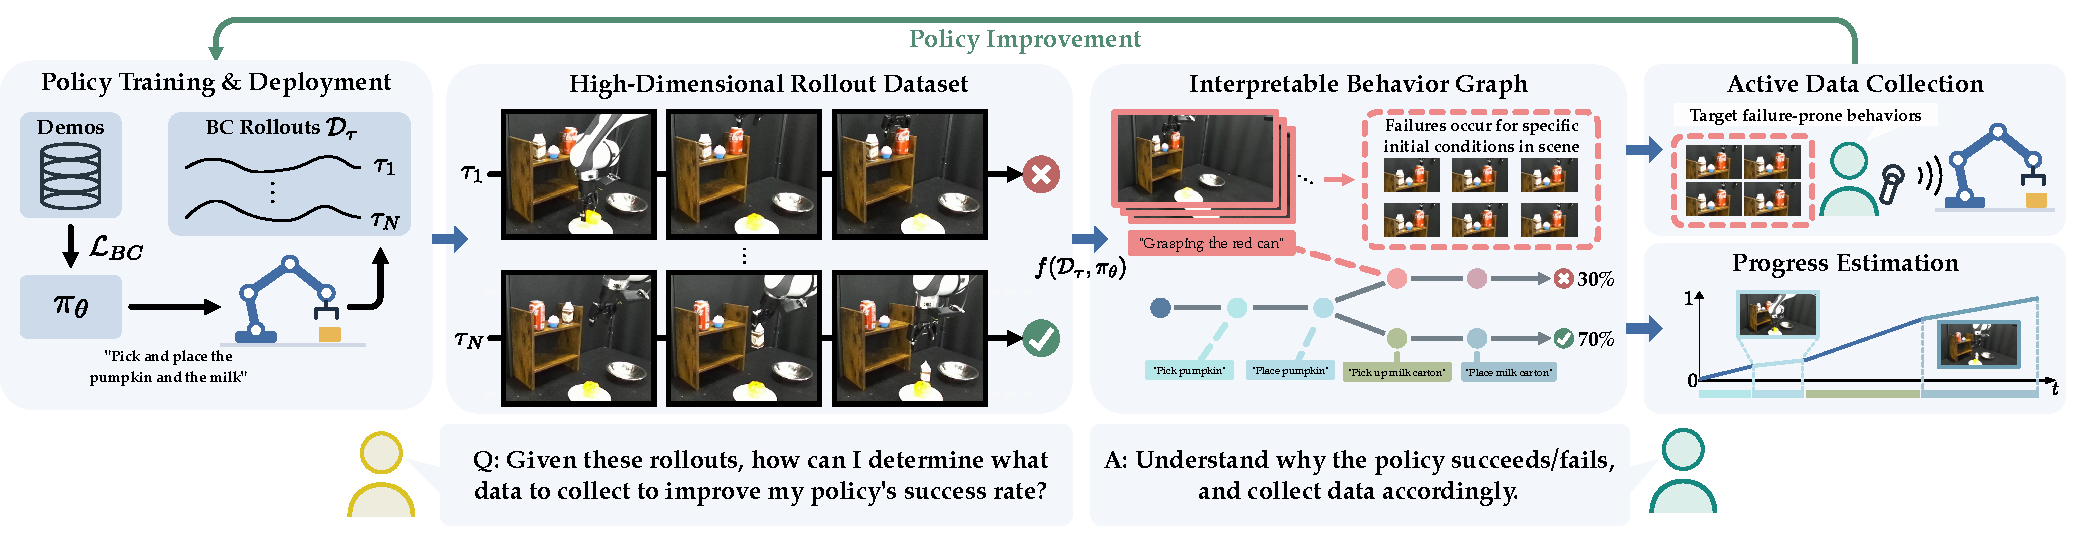
\includegraphics[width=\textwidth]{figures/fig1_updated.pdf}
           \captionof{figure}{\small Behavior graphs compress deployment rollouts into an interpretable representation of robot behavior and outcomes. Data collectors and researchers can use this structure to identify failure modes and guide targeted data collection, closing the policy improvement loop. Behavior graphs are a useful representation beyond interpretability, enabling state-of-the-art progress estimation zero-shot without any additional model training.}
           \label{fig:title_figure}
        \end{center}
    }]
}


\begin{document}
\nocite{IEEEexample:BSTcontrol}
% paper title
\title{\LARGE \bf Behavior Graphs: Unsupervised Graph Structures for Interpreting Robot Deployment Data}

% Alternatives
% \title{Steering the Data Flywheel: Interpretable Behavior Graphs for Imitation Learning}

% \author{Author Names Omitted for Anonymous Review [Paper ID: 3627]}

\newcommand{\authorhref}[3][black]{\href{#2}{\textcolor{#1}{#3}}}
\author{
    \bfseries
    \authorhref{http://erikbr01.github.io/}{Erik Bauer}\textsuperscript{1},\,\,
    \authorhref{https://jakob-thumm.com/}{Jakob Thumm}\textsuperscript{1},\,\,
    \authorhref{http://agiachris.github.io/}{Christopher Agia}\textsuperscript{1},\,\,
    \authorhref{https://rohansinha.nl/}{Rohan Sinha}\textsuperscript{1}\\ \bfseries
    \authorhref{https://hamrel-cxu.github.io/}{Chen Xu}\textsuperscript{3},\,\,
    \authorhref{https://harukins.github.io/}{Haruki Nishimura}\textsuperscript{3},\,\,
    \authorhref{https://web.stanford.edu/~bohg/}{Jeannette Bohg}\textsuperscript{1},\,\,
    \authorhref{https://profiles.stanford.edu/marco-pavone}{Marco Pavone}\textsuperscript{1,2},\,\,
    \authorhref{https://mashaitkina.weebly.com/}{Masha Itkina}\textsuperscript{3}\\\vspace{-8pt}\\
    \textsuperscript{1}\href{https://www.stanford.edu/}{Stanford University},
    \textsuperscript{2}\href{https://www.nvidia.com/en-us/research/}{NVIDIA Research},
    \textsuperscript{3}\href{https://www.tri.global/}{Toyota Research Institute}
    % \vspace{-18pt}
}%

\maketitle
% \IEEEpeerreviewmaketitle

\begin{abstract}
Data flywheels promise continuous improvement via insights from deployment data. However, robot deployments create large volumes of high-dimensional rollout data that is difficult to interpret and thus extract actionable insights from. To facilitate data flywheels for robotic manipulation, we propose behavior graphs, which compress policy rollouts into a single interpretable, directed graph. We construct the graphs by identifying similar behavior modes across rollouts, connecting the behaviors temporally, and finally linking them to outcomes. In a user study on three real-world tasks, 16 of 18 participants preferred behavior graphs to browsing rollout videos, reaching comparable conclusions with 40.3\% lower perceived temporal demand and 37.6\% lower effort. Beyond facilitating interpretability for deployment data, behavior graphs are capable progress predictors: across 43 rollout collections they raise value-order correlation from 0.769 to 0.945 and halve the mean absolute error of the strongest baseline. As the number of deployed robots grows, behavior graphs introduce the structure needed to interpret and reason about deployment data at scale. We open-source our code, data, and an interactive website demo at \href{https://try.behavior-graphs.com}{try.behavior-graphs.com}.
\end{abstract}


%===============================================================================
\section{Introduction}

Imitation learning has become a standard approach for training robotic manipulation policies~\cite{chi_diffusion_2023,zhao_learning_2023}. As policies move toward real-world deployment, improving them after initial training relies on the \emph{data flywheel}: deploy the policy, observe its rollout behavior, collect new demonstrations that address observed shortcomings, and retrain. Closing this loop effectively is difficult. Operators must identify not just that a policy fails, but which execution strategies are responsible, whether those failures stem from missing or low-quality training data, and what new demonstrations would meaningfully change the policy's behavior distribution. Without a structured account of policy behavior, these decisions reduce to intuition. As robots move from labs to deployments, the amount of generated rollout data will rapidly grow, and new methods are needed to enable reasoning about deployment data at scale to close the data flywheel loop.

Most existing works that attempt to learn from policy rollouts focus on direct policy improvement rather than generating interpretable insights. Data curation methods identify which existing demonstrations to discard~\cite{agia_cupid_2025, zhang_scizor_2025, chen_sarm_2025, intelligence2025pi06vlalearnsexperience}, but not which demonstrations to collect next. While red-teaming approaches~\cite{karnik2024embodied, majumdar2025predictive} can generate valuable insights about failure modes of a policy, they rely on actively steering policy inputs to cause failures, which is useful for finding weaknesses in a controlled setting, but may overly represent pessimistic scenarios compared to typical deployment settings. Active data collection approaches such as DAgger~\cite{kelly2019hgdaggerinteractiveimitationlearning, ross_reduction_2011} are effective, but expensive to scale, as they require constant monitoring and human experts to collect recovery data. None of these methods gives operators a way to interpret and act upon the autonomous rollout data that a robot deployment produces.

We address this gap with \emph{behavior graphs}, a representation that compresses policy rollouts into an interpretable directed graph~(Fig.~\ref{fig:title_figure}). Nodes in a behavior graph correspond to semantic behavior modes, which are connected by edges that represent the transition probabilities between different behaviors and rollout outcomes. Construction is unsupervised; we represent rollout segments with their policy embeddings and cluster them into behavioral modes. By exposing how different behavioral modes are connected to each other and success or failure across many rollouts, behavior graphs enable operators to easily identify where, when and how a policy fails, and thus guide data collection efforts accordingly. In a user study, this lowers perceived temporal demand by 40.3\% and effort by 37.6\% against a video browser, without changing the conclusions operators reach. Furthermore, with a lightweight model fit on top of the graphs, we obtain state-of-the-art (SOTA) progress estimation across 43 rollout collections, improving value-order correlation from 0.769 to 0.945 and more than halving mean absolute error against the strongest baseline, demonstrating that behavior graphs can serve as a potent representation beyond interpretability.

Our contributions are threefold:
\begin{itemize}
    \item A methodology for unsupervised behavior graph construction, with an ablation over representation and reduction choices across 3 tasks.
    \item A user study with three real-world tasks in which 16 of 18 operators prefer the graph over videos of rollouts, and perceived temporal demand and effort drop by 40.3\% and 37.6\% while data collection decisions remain comparable.
    \item A lightweight model fit on top of the graph to perform progress estimation, outperforming VLM- and learning-based baselines on all correlation and error metrics across 43 diverse datasets.
\end{itemize}

%===============================================================================
\section{Related Work}

\subsubsection{Identifying behavior from policies and trajectories} VLA hidden activations encode executed behaviors and can be used for steering~\cite{swann_sparse_2026, jin_eventgrounded_2026}, and unsupervised subtask segmentation~\cite{blank2026sparc, yang_unsupervised_2025, wang_grounding_2024} has been applied to skill transfer and retrieval~\cite{sharma_robosubtasknet_2026, memmel_strap_2025, chen_backbone_2025}. These works recover behavioral structure from policies and trajectories, but do not connect the identified behaviors to each other, nor use them to inform what data to collect next.

\subsubsection{Representing policies as graphs} Zahavy et al.~\cite{zahavy_graying_2016} and Topin et al.~\cite{topin_generation_2019} both abstract low-dimensional RL policies into behavioral MDPs, clustering deep Q-network representations in one case and grouping states by feature importance in the other. Graph structures can also be utilized as controllers: behavior trees~\cite{iovino_survey_2022} are authored by hand and imposed on a control architecture, while Pan et al.~\cite{pan2026emergentneuralautomatonpolicies} extract automaton structure from visuomotor trajectories to construct a policy. While these works share the motivation of utilizing graph-based structures to represent policy behaviors, their use case revolves around control rather than data collection or progress estimation.

\subsubsection{Policy improvement from deployment data} Curation methods use policy rollouts to score and reweight existing training data, whether through influence functions, self-supervised criteria, or learned value functions~\cite{agia_cupid_2025, zhang_scizor_2025, intelligence2025pi06vlalearnsexperience}, but do not reason about which data to collect next. Red-teaming approaches~\cite{karnik2024embodied, majumdar2025predictive} actively attempt to break the policy by assuming control over its observations and actively steering them towards failure-inducing regions, which is not representative of the typical deployment setting for robots that we consider. Variants of DAgger~\cite{ross_reduction_2011, kelly2019hgdaggerinteractiveimitationlearning} rely on experts monitoring policies for interventions and collecting failure recovery data, which is effective, but costly to scale. Zha et al.~\cite{zha_guiding_2025} guide collection by measuring performance scaling over coarse, manually-defined environmental factors.

\subsubsection{Progress estimation} Progress estimators support rollout analysis and reward modeling. Stage-conditioned estimators are interpretable, but require hand-annotated subtasks~\cite{chen_sarm_2025, kim2025subtask}. Generalist progress estimators such as Robometer~\cite{liang_robometer_2026} and TOPReward~\cite{chen_topreward_2026} need no task-specific training, but their accuracy varies widely across domains. We keep the stage-conditioned formulation of SARM~\cite{chen_sarm_2025}, but read the stages off a graph built from the policy's own rollouts, requiring no annotation.



%===============================================================================
\section{Methodology}

We first introduce methodology for unsupervised behavior graph construction, followed by how graphs can be used for active data collection and progress estimation.

\subsection{Behavior Graph Construction}

\begin{figure*}
  \vspace{10pt}
  \begin{center}
    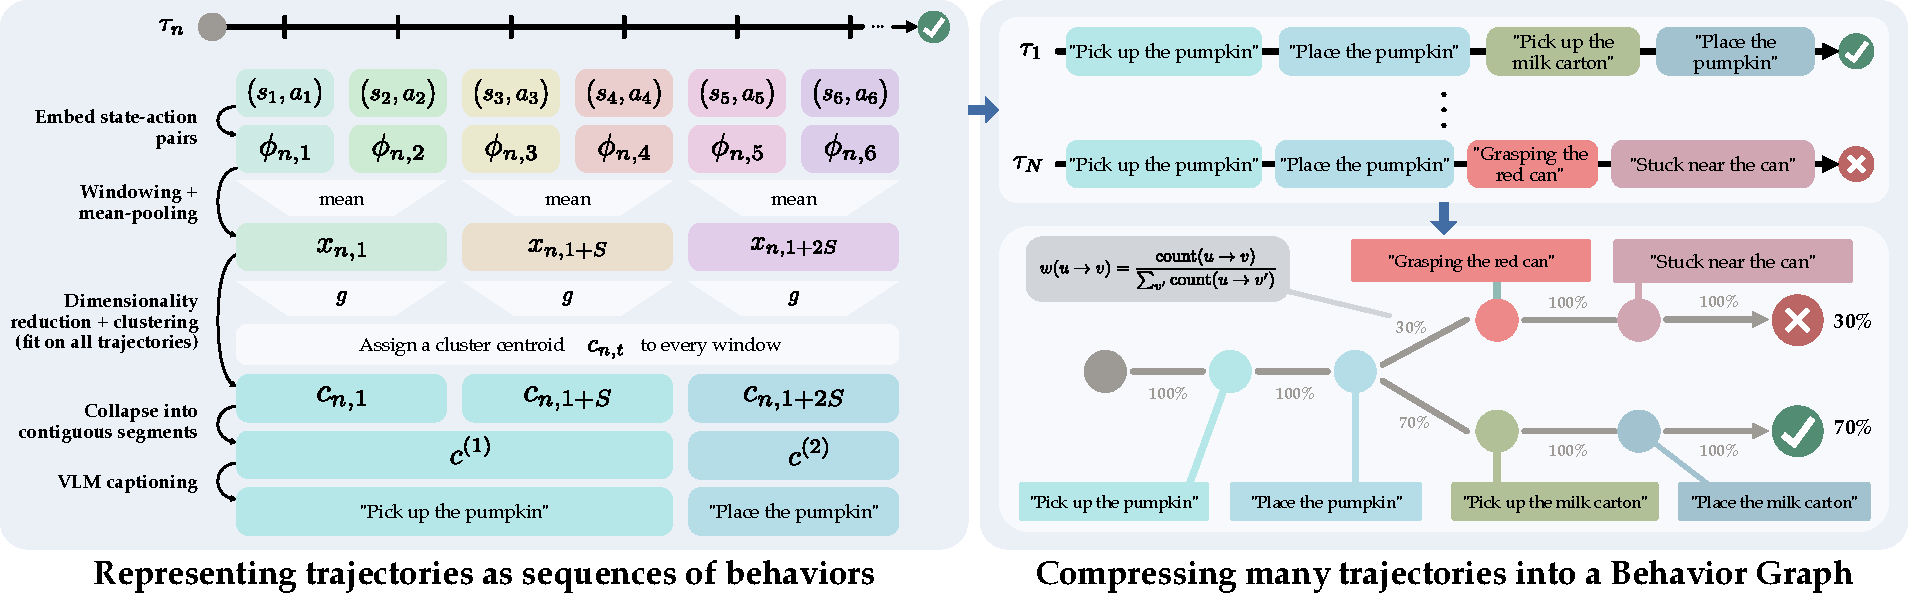
\includegraphics[width=\linewidth]{figures/fig2_updated.pdf}
  \end{center}
  \caption{\small Behavior graph construction. Timestep features are pooled over temporal windows, reduced in dimensionality, and clustered into shared behavior modes. Consecutive assignments to the same mode are collapsed into segments. The resulting sequences define a directed graph with empirical transition probabilities. VLM-generated labels obtained via contact sheets describe the discovered modes.}
  \label{fig:behavior_graph_construction}
\end{figure*}

We are given a set of trajectories $\rolloutset = \{\rollout_1, \ldots, \rollout_N\}$, where each trajectory $\rollout_n = \bigl((s_1, a_1), \ldots, (s_{T_n}, a_{T_n})\bigr)$ is a sequence of state-action pairs of length $T_n$. Trajectories are either policy rollouts, whose actions are sampled from a policy $\pi_\theta(a \mid s)$, or training demonstrations, whose actions are labeled by an expert. Each trajectory is annotated with a binary outcome $o(\rollout) \in \{\successnode, \failnode\}$. Finally, we assume access to an embedding function $f$ that maps a state-action pair to a vector in $\mathbb{R}^d$. The construction of the behavior graph follows the seven stages illustrated in Fig.~\ref{fig:behavior_graph_construction}: embedding trajectories, temporal aggregation, dimensionality reduction, clustering, segment collapsing, graph construction, and VLM annotation.

\begin{figure}
\vspace{10pt}
    \centering
    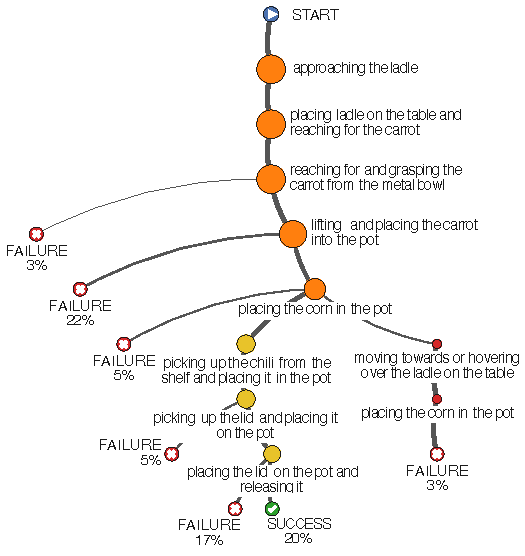
\includegraphics[width=0.95\linewidth]{figures/cooking_tree_height_compressed.pdf}
    \caption{\small Behavior graph for the cooking task of our user study~(Sec.~\ref{sec:user_study}). The larger the node, the higher the visitation count. Node colors indicate success likelihood (increasing from red to green), while all terminal nodes are annotated with their likelihoods.}
    \label{fig:set_table_behavior_graph}
\end{figure}

\paragraph{Embedding trajectories}
We first embed every timestep of every trajectory as \(\phi_{n,t} = f(s_t, a_t) \in \mathbb{R}^d\). The choice of \(f\) determines what notion of similarity the graph is built on, and is the design decision with the largest effect on the resulting graph. We consider three families: policy embeddings, where \(f\) returns the output of the observation encoder of \(\pi_\theta (a \mid s)\); state-action features, where \(f(s,a) = \begin{bmatrix} s^\top & a^\top \end{bmatrix}^\top\); and embeddings produced by pretrained visual encoders such as DINOv3. Unless otherwise stated, policy embeddings come from flow matching policies.

\paragraph{Temporal aggregation}

Typically, behaviors span multiple timesteps. To alleviate potential noise in the embedding space, we aggregate over short temporal windows. Given a window width \(W\) and a stride \(S\), trajectory \(\rollout_n\) contributes the windows starting at \(t \in \{1, 1 + S, 1 + 2S, \ldots\}\) with \(t + W - 1 \leq T_n\). Each window is represented by mean-pooling the embeddings from all its timesteps:

\begin{equation}
  x_{n,t} = \frac{1}{W} \sum_{k=t}^{t+W-1} \phi_{n,k}
  \label{eq:slice_embed}
\end{equation}

Applying this to all trajectories yields the set of windows \(\mathcal{X} = \{x_{n,t}\}\), which contains all windows from all rollouts.

\paragraph{Dimensionality reduction and clustering}

To facilitate downstream clustering, we apply dimensionality reduction \(g: \mathbb{R}^d \to \mathbb{R}^{d_\text{low}} \) to all elements in \(\mathcal{X}\). Like the embedding function, \(g\) is a design choice rather than a fixed part of the method, and we evaluate three instantiations: UMAP, which preserves local neighborhood structure nonlinearly; PCA, which is linear and preserves directions of global variance; and the identity map as control.

Clustering partitions the set of reduced windows \(\mathcal{Z} = g(\mathcal{X})\) into \(K\) groups, using \(K\)-means. We henceforth refer to these groups as behaviors \(\mathcal{C} = \{c_1, \ldots, c_K\}\), and represent them by their centroid. We write \(c_{n,t} \in \mathcal{C}\) for the behavior assigned to window \(x_{n,t}\).

\paragraph{Segment collapsing}
After clustering, we obtain a behavior mode assignment for all windows across all trajectories. Within one trajectory, most behaviors typically span multiple consecutive windows. For each trajectory, we merge consecutive windows carrying the same behavioral assignment into a single \emph{segment}, reducing the trajectory to a compact sequence
\begin{equation}
  \sigma_n = \bigl(c^{(1)}, c^{(2)}, \ldots, c^{(L_n)}\bigr), \quad c^{(l)} \in \mathcal{C}, \quad c^{(l)} \neq c^{(l+1)}
  \label{eq:collapsed}
\end{equation}
of the \(L_n\) distinct behaviors.

\paragraph{Graph construction}
The collapsed sequences define a directed graph \(G = (V, E)\) over behaviors and outcomes, with node set $V = \{\textsc{Start}\} \cup \mathcal{C} \cup \{\successnode,\, \failnode\}$ adding a source node and the two outcome nodes to the behaviors. Each sequence \(\sigma_n\) contributes an edge \(\textsc{Start} \to c^{(1)}\), the inter-behavior edges \(c^{(l)} \to c^{(l+1)}\), and a terminal edge \(c^{(L_n)} \to o(\rollout_n)\) into the trajectory's outcome. Since collapsing leaves no two adjacent behaviors equal, \(E\) contains no self-loops. In addition, every edge carries the probability of taking that transition, estimated from the counts \(\mathrm{count}(u \to v)\) accumulated over all trajectories and normalized over the outgoing edges of its source:
\begin{equation}
  w(u \to v) = \frac{\mathrm{count}(u \to v)}{\sum_{v'} \mathrm{count}(u \to v')}.
  \label{eq:edge_weights}
\end{equation}

These weights assume that transitions are first-order Markovian, and whether that assumption holds is not always clear. We have found prefix trees to be a viable alternative: a node is a path prefix, so execution modes that visit the same behaviors in different orders stay distinct and no Markov assumption is needed. However, prefix trees give up the graph's bound on node count, growing instead with the number of distinct orderings the policy exhibits. Nothing in the remainder of our methodology relies on the Markov assumption, so the choice between the two reduces to a preference in visualization.

\paragraph{VLM annotation}
Captioning the discovered behaviors \(\mathcal{C}\) makes it easier to understand the graph at a glance, rather than having to inspect all behaviors to understand their meaning. To enable automatic captioning by VLMs, we utilize contact sheets. A contact sheet for a behavior \(c \in \mathcal{C}\) is a \(j \times k\) grid of images, which samples \(j\) segments that were assigned to \(c\), and represents each segment with \(k\) uniformly sampled images~(Fig.~\ref{fig:behavior_graph_construction}). The VLM receives the contact sheet together with a text description of the graph topology, and optionally, a task instruction as specified by the user. In a first pass, the VLM generates a caption \(\ell_c\) for every behavior. In a second pass, it reflects on the captions, evaluates global coherency, and corrects them if necessary.
 

\subsection{Use Cases}
\label{subsec:use_cases}
 
We consider two use cases for behavior graphs: active data collection and progress estimation. For data collection, we read quantities directly off the graph, while for progress estimation, we fit a lightweight model on top of it.
 
\subsubsection{Active data collection}
To support failure analysis, the tree exposes distinct execution modes and their outcomes as separate branches, and branches whose likelihood falls below a user-defined threshold can be folded in or pruned.
 
Two quantities follow directly from the graph and let operators reason about failure at the level of individual behaviors or entire execution strategies. The \emph{success likelihood} of a behavior \(c\) is the fraction of trajectories that visited \(c\) and ended in success:
\begin{equation}
  p_\text{succ}(c) = \frac{\bigl|\{n : c \in \sigma_n,\; o(\rollout_n) = \successnode\}\bigr|}{\bigl|\{n : c \in \sigma_n\}\bigr|}
  \label{eq:psucc}
\end{equation}
This isolates failure-prone behaviors independently of where in the execution they occur. When read together with the visitation count \(\bigl|\{n : c \in \sigma_n\}\bigr|\), it identifies clear data collection targets: behaviors that are both frequently visited and result in failure. Visually, we show the success likelihood via a color gradient for nodes in the graph, ranging from red for \(p_\text{succ} = 0\) to green for \(p_\text{succ} = 1\)~(Fig.~\ref{fig:set_table_behavior_graph}). The visitation count is visualized via the radius of the circle representing the node in the graph. Furthermore, we can consider entire paths in addition to isolated behaviors. The likelihood of a path \(\rho = \bigl(\textsc{Start}, c^{(1)}, \ldots, c^{(L)}, o\bigr)\) is the product of its edge weights,
\begin{equation}
  P(\rho) = \prod_{l=0}^{L} w\bigl(c^{(l)} \to c^{(l+1)}\bigr),
  \label{eq:pathprob}
\end{equation}
with \(c^{(0)} = \textsc{Start}\) and \(c^{(L+1)} = o\). On the tree both quantities are read per branch instead. For a prefix tree, we write \(\rho \preceq \sigma_n\) when \(\rho\) is a prefix of rollout \(n\)'s behavior sequence, and \(N(\rho) = \bigl|\{n : \rho \preceq \sigma_n\}\bigr|\) for the rollouts that followed it, a branch's likelihood is \(P(\rho) = N(\rho)/N\) and its success likelihood is \(p_\text{succ}(\rho) = \bigl|\{n : \rho \preceq \sigma_n,\; o(\rollout_n) = \successnode\}\bigr| / N(\rho)\). 

Ranking paths by \(P(\rho)\) surfaces the policy's dominant execution strategies, so that operators can see which failure modes occur most often and allocate collection budgets accordingly. The added temporal context of analyzing paths instead of individual behaviors can be helpful in cases where the root cause of a failure lies in a behavior that is upstream in the graph rather than in the behavior that occurs immediately before failure.

Furthermore, we make the graphs interactive: in the web-based interface, users can click on nodes or transitions to see videos of all episodes that went through the node or transition, starting from the point in time where the behavior or the behavioral transition occurred. Thus, users can pinpoint high-level failures by considering either the node- or path-level failure candidates, and then analyzing the rollouts that have been grouped into that particular failure-prone behavior mode.
 
\subsubsection{Progress Estimation}
\label{sec:progress_method}

Estimating how far a rollout progressed through its task can be useful for analyzing deployments retroactively. Such estimators are typically learned end-to-end from trajectories and progress labels. SARM~\cite{chen_sarm_2025} instead conditions progress on which subtask a rollout occupies, which makes the estimate interpretable but requires the subtasks to be annotated by hand. We adopt this formulation and take the subtasks from the behaviors the graph discovers, removing the annotation requirement.
 
Each behavior in the graph thus plays the role of a subtask. Progress is modeled for individual behaviors as a linear function throughout the duration of a behavioral segment. Total progress in a rollout is modeled as a piecewise linear function composed of the individual progress models per behavior the rollout is in. The expected progress within a behavior \(c\) is \(\bar{p}_c = \beta_c + \alpha_c \, \bar{t}\), where \(\bar{t} \in [0, 1]\) is the elapsed normalized time within the behavior. To fit the individual progress models for all behaviors, we compute \(\alpha_c\) and \(\beta_c\) from a dataset of successful trajectories (either training demonstrations or successful rollouts) that we fit a behavior graph on.
 
The slope \(\alpha_c\) of the progress model is the expected fraction of a trajectory that \(c\) occupies across all trajectories,
\begin{equation}
  \alpha_c = \avg_n \frac{\bigl| \{ t : c_{n,t} = c \} \bigr|}{\lvert \mathcal{X}_n \rvert},
  \qquad \textstyle\sum_{c \in \mathcal{C}} \alpha_c = 1,
  \label{eq:stage_span}
\end{equation}
with \(\mathcal{X}_n \subset \mathcal{X}\) the windows of \(\rollout_n\) used to build the behavior graph. The intercept of the progress model is the total slope of all behaviors preceding \(c\). Ordering \(\mathcal{C}\) by mean normalized time of occurrence \(t / T_n\), we accumulate
\begin{equation}
  \beta_{c_k} = \beta_{c_{k-1}} + \alpha_{c_{k-1}},
  \qquad \beta_{c_1} = 0.
  \label{eq:stage_base}
\end{equation}
To score a new trajectory, we assign its windows to behaviors of the initial graph we fit, collapse them into segments, and evaluate \(\bar{p}_c\) on each segment to obtain the expected progress for each behavior.

%===============================================================================
\section{Experiments}

\begin{figure*}[!t]
    \centering
    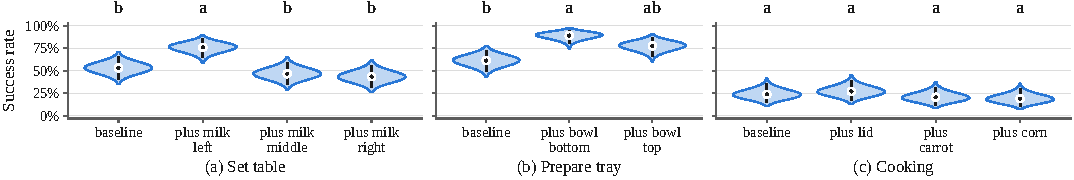
\includegraphics[width=\linewidth]{figures/policy_comparison.pdf}
    \caption{\small 
    Targeted data helps only when it addresses the policy's most frequent failure mode. Estimated success rates~\cite{barreiros_careful_2026} of the baseline policy and of policies retrained with 30 additional demonstrations for each candidate data-collection strategy, on three real-world DROID tasks. In {\em Set table\/}, only demonstrations with the milk carton on the left (the position missing from the baseline training data) improve performance. In {\em Prepare tray\/}, bottom-shelf bowl demonstrations improve over the baseline. In {\em Cooking\/}, no single-subtask strategy makes a significant difference. Violins show the Bayesian posterior over each policy's success rate (uniform Beta prior). Dots and bars mark the posterior mean and interval. Letters above each column~\cite{piepho2004algorithm} summarize pairwise significance tests within a task~\cite{snyder2025your}: two policies that share a letter are not significantly different; policies with no letter in common are.
    Tests follow~\cite{snyder2025your} with family-wise error rate (FWER)  controlled at 5\%, and 60 policy rollouts to estimate each posterior.   
}
    \label{fig:overall}
    % \vspace{}
\end{figure*}

\begin{figure*}
    \centering
    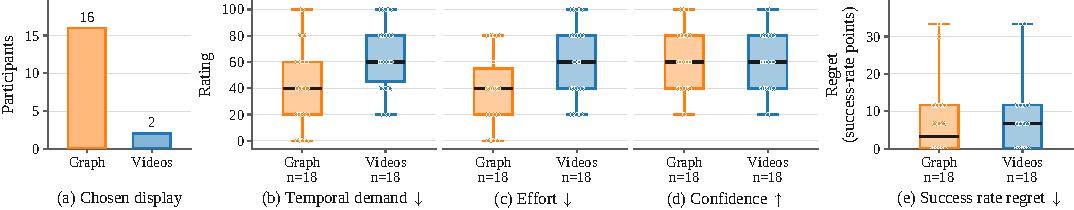
\includegraphics[width=\linewidth]{figures/study_answers.pdf}
    \caption{\small
    Behavior graphs make rollout analysis less demanding without changing the decisions users reach. Responses from our user study ($n=18$).  
    (a)~When free to choose a display for the third task, 16 of 18 participants picked the behavior graph over the video browser. (b-d)~Self-reported ratings (0-100, in steps of 20) after analyzing a task with each display: the graph lowers perceived temporal demand~(b) and effort~(c), while confidence in the chosen data-collection strategy is unchanged~(d). Boxes span the interquartile range with the median marked, whiskers span min/max values; dots are individual ratings. 
    (e) The success rate regret (i.e., the gap between the best retrained policy in Fig.~\ref{fig:overall} and the one the participant selected) 
    % Lower means a better choice. 
    is similar for graph and videos. Arrows indicate whether higher~($\uparrow$) or lower~($\downarrow$) is better. Tab.~\ref{tab:study-adjusted} reports the corresponding effects adjusted for task, stage, and experience.
    }
    \label{fig:user_study_results}
\end{figure*}

We evaluate behavior graphs for active data collection and progress estimation, and ablate the graph construction methodology. We investigate the following questions:

\textbf{Q1: How do behavior graphs impact decision-making processes for failure analysis and data collection?} In a user study on three real-world tasks on a DROID~\cite{khazatsky2024droid} setup, participants analyze policy rollouts presented either as a behavior graph or an unstructured video browser, rank failure modes, and select data collection strategies. 
We track metrics for the decision-making process and its downstream outcomes, obtained by collecting data for each candidate data collection strategy and retraining the policy on it.

\textbf{Q2: How do behavior graphs compare to specialized progress estimators?} We test whether the graph is a useful representation beyond interpretability, by comparing our graph-based progress estimator against SOTA baselines.

\textbf{Q3: Which graph construction choices matter, and how sensitive is graph quality to them?} We validate how we construct behavior graphs in an ablation study on three real-world tasks, and inspect graphs built for six policy architectures across simulated and real tasks.

\subsection{Behavior Graphs for Active Data Collection (Q1)}
\label{sec:user_study}

We evaluate the impact of behavior graphs on decision-making processes for data collection. Each user analyzes policy rollouts for three tasks in random order. 
The first two tasks expose the user to two visualizations in random order: one task is shown as a behavior graph, the other through a video browser that allows the user to explore all rollout videos, filtered by success or failure. To speed up exploration for the video browser, we show 6 rollouts at a time. 
For the third task, users choose their preferred visualization, which we take as the preference measure.

\subsubsection{Real-World Tasks}

The three tasks are chosen to expose distinct failure modes. In \emph{set table}, the robot places a toy pumpkin, then a chocolate milk carton taken from a shelf holding two distractors. To induce a data coverage failure, we train the baseline on all permutations of the three shelf objects except those with the carton on the left. In \emph{prepare tray}, the robot slides a tray out from under a shelf, places a bowl from the top or bottom of the shelf onto it, and picks up a fork. Sliding the tray is non-prehensile, which stresses subtask segmentation, and the bowl and fork demand precise gripper placement. Failures spread more evenly here and stem largely from the precision the last two subtasks require, occurring slightly more often on the bottom-shelf bowl, whose grasp demands a more complex motion given the robot's kinematics. In \emph{cooking}, the robot clears a ladle from a pot, transfers a toy corn, carrot, and chili into it from a bowl and a shelf, and finally places the lid on the pot.

The candidate data collection strategies are the possible milk carton positions in \emph{set table}, the bowl's shelf height in \emph{prepare tray}, and individual subtasks in \emph{cooking}. Baseline policies are trained on 120 demonstrations for \emph{set table} and \emph{prepare tray}, and 200 for \emph{cooking}. 
Fig.~\ref{fig:overall} reports success rate from training on baseline data plus 30 added demonstrations for each data collection strategy.
In \emph{set table}, only the held-out carton position improves performance, as the alternatives add data for conditions the policy already handles. The bottom-shelf bowl is likewise the better choice in \emph{prepare tray}, by a smaller margin. In \emph{cooking}, 30 demonstrations targeted at a single subtask produced no significant difference in success rate between the options. 


\subsubsection{Metrics}

For each task, users are asked to rank the three most likely failure modes and select the data strategy they believe will most improve policy performance. A strategy is a class of additional demonstrations to collect, specified as either an initial condition, such as an object's starting position, or a subtask. Users choose from predefined options for both questions. Afterward, users rate the effort it took to answer these questions, perceived temporal demand, and confidence from 0 to 100 in increments of 20.


\subsubsection{Analysis}

All analyses use the first two randomized stages from \(N=18\) participants, yielding 36 responses; the third stage contributes only the preference measure. For each outcome, we fit a linear mixed-effects model,
\begin{equation}
    y_{ij} = \beta_0 + \beta_G G_{ij} + \beta_T T_{ij} + \beta_S S_{ij} + \beta_E E_i + b_i + \epsilon_{ij}
    \label{eq:user-study-mixed-model}
\end{equation}

% \begin{align}
% y_{ij} &=
% \beta_0 + \beta_G G_{ij}
% + \tau_{T_{ij}} + \beta_S S_{ij}
% + \beta_E E_i + b_i + \epsilon_{ij}, \\
% T_{ij} &\in
% \{\text{Set table}, \text{Prepare tray}, \text{Cooking}\}, \\
% G_{ij} &=
% \begin{cases}
% 1, & \text{if participant \(i\) uses a behavior graph at stage \(j\)}, \\
% 0, & \text{if they use videos},
% \end{cases} \\
% S_{ij} &=
% \begin{cases}
% 1, & \text{if \(j=2\)}, \\
% 0, & \text{if \(j=1\)},
% \end{cases} \\
% E_i &\in \{0,1,2,3,4\}, \qquad
% b_i \sim \mathcal{N}(0,\sigma_p^2), \qquad
% \epsilon_{ij} \sim \mathcal{N}(0,\sigma_\epsilon^2).
% \label{eq:user-study-mixed-model}
% \end{align}

Here, \(y_{ij}\) is participant \(i\)'s rating at stage \(j\). \(G_{ij}\), \(T_{ij}\), and \(S_{ij}\) denote visualization, task, and study stage, respectively. \(E_i\) is self-reported data-collection experience. The participant-specific random intercept \(b_i \sim \mathcal{N}(0,\sigma_p^2)\) captures differences in how participants use the rating scale. We treat the six-point 0--100 ratings as continuous and report estimated marginal means (EMMs) per visualization, together with the graph effect \(\beta_G\) as their difference and its 95\% credible interval (CrI). Each EMM averages over task, study stage, and experience, with participant intercepts set to zero.

To evaluate data-collection decisions, we use success rate regret, \(r = s_{\max} - s_{\text{chosen}}\), where \(s_{\max}\) is the highest retrained-policy success rate among the data-collection options available for that task and \(s_{\text{chosen}}\) is the success rate obtained from the option selected by the participant. Intuitively, a lower success rate regret implies the selection of a better data collection strategy (e.g., zero regret corresponds to selecting the best available option). Rating outcomes are reported in rating points and regret in terms of success rate.

\subsubsection{Results}

Behavior graphs make rollout analysis faster and easier without changing what users conclude~(raw ratings in Fig.~\ref{fig:user_study_results}, estimated marginal means in Tab.~\ref{tab:study-adjusted}). 
In particular, the graph reduces perceived temporal demand by 26.1 points and effort by 22.9 points compared to videos (40.3\% and 37.6\% relative decrease).  
User confidence in the selected data collection strategy and the resultant success rate regret (averaged across tasks) show no reliable difference, indicating that the graph incurs negligible information loss relative to video data for the purposes of active data collection.
Overall, 16 of 18 participants (89\%) chose the graph for the self-selected third task, indicating strong user preference. 
% Confidence and success rate regret show no reliable difference. 

% Fig.~\ref{fig:overall} shows the retrained policies behind that metric. In \emph{set table}, only the held-out carton position improves performance, as the alternatives add data for conditions the policy already handles. The bottom-shelf bowl is likewise the better choice in \emph{prepare tray}, by a smaller margin. In \emph{cooking}, 30 demonstrations targeted at a single subtask produced no significant difference in success rate between the options. 

% Overall, 16 of 18 participants (89\%) chose the graph for the self-selected third task, indicating strong user preference. 

\begin{table}[t]
  \centering
  \caption{\small Effect of the behavior graph after adjusting for task, study stage, participant experience, and individual differences in scale use. We report estimated marginal means per visualization from the mixed-effects model~(Eq.~\ref{eq:user-study-mixed-model}) and their difference. The reductions in perceived temporal demand and effort persist under adjustment, confidence and success rate regret are unchanged.
  }
  \label{tab:study-adjusted}
  \small
  \begin{tabular}{@{}lrrl@{}}
  \toprule
  Outcome                      & Graph  & Videos & Difference [95\% CrI] \\
  \midrule
  Temporal demand $\downarrow$ & $38.7$ & $64.8$ & $-26.1$ $[-38.4, -14.0]$ \\
  Effort $\downarrow$          & $38.1$ & $61.0$ & $-22.9$ $[-37.7, -7.8]$ \\
  Confidence $\uparrow$        & $61.3$ & $58.8$ & $+2.5$ $[-9.8, +15.5]$ \\
  Success rate regret $\downarrow$ & $7.9$  & $7.0$  & $+0.9$ $[-6.1, +8.5]$ \\
  \bottomrule
  \end{tabular}
\end{table}


\subsection{Behavior Graphs for Progress Estimation (Q2)}

\subsubsection{Data, Baselines, and Metrics}

We evaluate behavior graphs as backbones for progress estimation via the methodology described in Sec.~\ref{subsec:use_cases}. We consider 43 rollout datasets, spanning tasks in simulation and the real-world taken from LIBERO~\cite{liu_libero_2023}, Robomimic~\cite{mandlekar_robomimic_2021}, MimicGen~\cite{mandlekar_mimicgen_2023}, and tasks from the real-world DROID setup. LIBERO rollouts were obtained with \(\pi_{0.5}\)~\cite{pi05_2025} (multi-task datasets) and the rest of the rollouts were obtained with flow matching policies (single-task datasets), using condition vectors as representation and UMAP for dimensionality reduction. We randomly sample 3 train/val/test splits: graphs are fit on the train split, hyperparameters are optimized on the validation split, metrics are reported for the unseen test splits, as averages over 3 train/validation/test splits.

We compare our method against two SOTA VLM-based progress estimators, Robometer~\cite{liang_robometer_2026} and TOPReward~\cite{chen_topreward_2026}, and against a baseline that fits an MLP on the same policy embeddings the graph is built on, which separates the contribution of the graph structure from that of the underlying representation. We report value-order correlation~(VOC), Kendall's $\tau$, mean absolute error against ground-truth progress, and AUC for the rollout outcome classification that the progress estimate induces.

\subsubsection{Results}

Averaged over all 43 datasets, behavior graphs achieve the best VOC, Kendall's $\tau$, and mean absolute error (see Tab.~\ref{tab:progress-by-rubric}), outperforming in 3/4 domains on VOC, 4/4 on $\tau$, 3/4 on the MAE. The only domain where a baseline leads on these metrics is LIBERO, where the MLP fit on the same policy embeddings is slightly ahead on VOC and mean absolute error. Baselines remain competitive on AUC, where Robometer is strongest on average. VLM-based models are capable at predicting outcomes, but predict progress with less fidelity. We demonstrate that given a trained policy and a dataset of successful trajectories, behavior graphs are a highly capable progress estimator despite not using neural networks of any sort and only minimal parameter learning. Furthermore, outperforming the MLP baseline, which operates on the same policy embeddings that the graph is built on, demonstrates that the temporal and behavioral structure imposed by the behavior graph is a helpful prior that significantly boosts performance over naive learning-based approaches.

\begin{table}
  \vspace{5pt}
  \centering
  \caption{\small Progress-estimation metrics over 43 datasets spanning 4 domains. On average, graph-based progress estimation outperforms all baselines in the fidelity of the prediction. In AUC, which measures success classification induced by the progress estimates, Robometer outperforms on average.}
  \label{tab:progress-by-rubric}
  \setlength{\tabcolsep}{3pt}
  \begin{tabular}{@{}llrrrr@{}}
  \toprule
  Domain (\#Datasets)                          & Method             & VOC $\uparrow$          & Kendall $\uparrow$         & MAE $\downarrow$           & AUC $\uparrow$\\
  \midrule
  \multirow{4}{*}{LIBERO (6)}        & Graph (ours) & 0.912          & \textbf{0.864} & 0.082          & 0.807 \\
                                     & MLP        & \textbf{0.940} & 0.861          & \textbf{0.068} & \textbf{0.864} \\
                                     & Robometer-4b       & 0.799          & 0.650          & 0.154          & 0.860 \\
                                     & TOPReward          & 0.433          & 0.329          & 0.259          & 0.664 \\
  \midrule
  \multirow{4}{*}{Real-world (19)} & Graph (ours) & \textbf{0.948} & \textbf{0.930} & \textbf{0.047} & \textbf{0.904} \\
                                     & MLP        & 0.731          & 0.564          & 0.173          & 0.782 \\
                                     & Robometer-4b       & 0.664          & 0.496          & 0.181          & 0.859 \\
                                     & TOPReward          & 0.736          & 0.572          & 0.192          & 0.674 \\
  \midrule
  \multirow{4}{*}{Robomimic (10)}    & Graph (ours) & \textbf{0.965} & \textbf{0.958} & \textbf{0.108} & 0.763 \\
                                     & MLP        & 0.682          & 0.565          & 0.198          & \textbf{0.871} \\
                                     & Robometer-4b       & 0.431          & 0.342          & 0.234          & 0.751 \\
                                     & TOPReward          & 0.478          & 0.359          & 0.308          & 0.767 \\
  \midrule
  \multirow{4}{*}{Mimicgen (8)}      & Graph (ours) & \textbf{0.936} & \textbf{0.907} & \textbf{0.078} & 0.595 \\
                                     & MLP        & 0.841          & 0.688          & 0.125          & 0.742 \\
                                     & Robometer-4b       & 0.646          & 0.495          & 0.224          & \textbf{0.789} \\
                                     & TOPReward          & 0.603          & 0.464          & 0.235          & 0.724 \\
  \midrule
  \midrule
  \multirow{4}{*}{Average (43)}    & Graph (ours) & \textbf{0.945} & \textbf{0.923} & \textbf{0.072} & 0.802 \\
                                   & MLP        & 0.769          & 0.629          & 0.155          & 0.804 \\
                                   & Robometer-4b       & 0.625          & 0.482          & 0.197          & \textbf{0.824} \\
                                   & TOPReward          & 0.609          & 0.469          & 0.236          & 0.700 \\
  \bottomrule
  \end{tabular}
\end{table}

%==============================================================================


\subsection{Ablation Study (Q3)}

We ablate the effect of several design decisions on graph construction quality across all three real-world tasks in our user study. We estimate ground truth subtask boundaries via gripper opening and closing as a heuristic. We split the datasets 60/20/20 for training, validation and test splits and evaluate graph construction via the proxy task of subtask segmentation. Similarly to progress estimation, graphs are fit on train, hyperparameters (including the number of behaviors~\(K\)) are optimized on val, and metrics are reported on the unseen test split. We use two metrics: \(F_1\), computed at an intersection-over-union (IoU) threshold of 0.75, and mean IoU for predicted segments that have been matched to a ground truth counterpart.

\subsubsection{Results}

Tab.~\ref{tab:ablation} sweeps three embedding representations against the three dimensionality reduction techniques. Averaged over reductions, policy embeddings lead on both metrics, at $F_1$ of $0.226$ against $0.132$ for proprioception and $0.113$ for DINOv3, and the best single cell on each metric is a policy-embedding row. The reduction yields no clear quantitative result, with the best setting differing by representation. Qualitatively, we find that policy embeddings under UMAP produce the most legible graphs.

\subsubsection{Does graph creation work across policies and tasks?}

Graph creation produces qualitatively coherent graphs across six policy classes (diffusion~\cite{chi_diffusion_2023} and flow matching policies, $\pi_{0.5}$~\cite{pi05_2025}, OpenVLA~\cite{kim_openvla_2024}, $\pi_0$-FAST, Foundry-VLA) on both short- and long-horizon tasks in simulation and the real world. We provide the resulting graphs on the interactive website. As most datasets have no subtask annotations, we cannot quantitatively assess graph quality for all datasets.

% \todo[inline]{this subsubsection is really qualitative only right now. still important imo to touch on generality, but hard to show quantitatively. keep this?}

%==============================================================================


\begin{table}[t]
\vspace{5pt}
\centering\small
\caption{\small Ablation study results for subtask segmentation. We report mean/std. over 3 datasets, and the mean/std for each representation averaged over all reductions. We report $F_1$ at 0.75 IoU threshold and the mean IoU over matched segments. On average, policy embeddings outperform proprioception and frozen DINOv3 features. While there is no clear quantitative conclusion for reductions, UMAP performs more consistently than the others and is what we use for our other experiments.}
\setlength{\tabcolsep}{4pt}
\begin{tabular}{@{}ll rr@{}}
\toprule
Representation & Reduction & $F_1(0.75)\uparrow$ & IoU$\uparrow$ \\
\midrule
\multirow{3}{*}{Proprioception}
  & none & $0.093${$\pm0.075$} & $0.523${$\pm0.061$} \\
  & PCA  & $0.120${$\pm0.121$} & $0.547${$\pm0.098$} \\
  & UMAP & $0.182${$\pm0.022$} & $0.598${$\pm0.033$} \\

  & \emph{mean} & $0.132 \pm 0.072$ & $0.556 \pm 0.063$ \\
\midrule
\multirow{3}{*}{Policy embeddings}
  & none & $\mathbf{0.264}${$\pm0.108$} & $0.633${$\pm0.048$} \\
  & PCA  & $0.254${$\pm0.121$} & $\mathbf{0.644}${$\pm0.059$} \\
  & UMAP & $0.160${$\pm0.031$} & $0.567${$\pm0.022$} \\
  & \emph{mean} & $0.226 \pm 0.086$ & $0.615 \pm 0.032$ \\
\midrule
\multirow{3}{*}{DINOv3}
  & none & $0.088${$\pm0.030$} & $0.462${$\pm0.029$} \\
  & PCA  & $0.082${$\pm0.023$} & $0.462${$\pm0.022$} \\
  & UMAP & $0.169${$\pm0.086$} & $0.566${$\pm0.088$} \\
  & \emph{mean} & $0.113 \pm 0.019$ & $0.497 \pm 0.014$ \\
\bottomrule
\end{tabular}
\label{tab:ablation}
\end{table}

\subsection{Discussion and Limitations}
 
On decision-making (Q1), behavior graphs compress deployment rollouts into a structure operators read faster, with less effort, and strongly prefer over rollout videos, while reaching comparable data collection decisions: neither confidence nor success rate regret differs reliably between the two. At the scale of our study, a well-informed operator reaches sound conclusions from videos alone, so the graph's observable value lies in how quickly they get there. We expect the gap to widen with the number of rollouts and behaviors, since the difficulty of reading videos scales with the size of a deployment while reading a graph does not.
 
As a representation beyond interpretability (Q2), the same structure supports progress estimation: a piecewise-linear readout on the discovered behaviors outperforms both VLM-based and learned estimators on correlation and error, without requiring the subtask segmentation annotations that comparable stage-aware estimators depend on. Its main limitation is that the readout, like in other estimators, is non-causal and would need adapting for monitoring during inference.
 
On construction (Q3), the chosen representation for graph creation has a significant impact on the results. While subtask segmentation is a proxy task, as interpretability cannot be easily evaluated, we find that the quantative results favoring policy embeddings are reflected in our qualitative experience, where policy embeddings typically lead to interpretable graphs. For the reduction, qualitative and quantitative findings are not always consistent: in practice, we utilize UMAP. The number of behaviors \(K\) also has a large impact on the graphs our methodology produces, though it is more of a user choice that defines the level of detail for interpretability. Overall, these limitations are largely related to subtask segmentation to construct graphs. We expect that as the spatial understanding of VLMs improves, they will be able to annotate subtasks reliably and cheaply enough to replace clustering altogether.

%===============================================================================
\section{Conclusion}

With behavior graphs, we aim to make large volumes of rollout data interpretable and actionable. Construction requires nothing beyond a trained policy and its rollouts, reusing representations the policy already provides. The resulting structures summarize policy behavior at a glance, even across hundreds of rollouts, and expose the failure modes that should drive the next round of data collection. In our study, operators reached the same conclusions from the graph as from rollout videos while spending markedly less perceived time and effort, and 16 of 18 chose it when given the option. Beyond serving as a visual summary, the structure imposed by behavior graphs benefits downstream tasks: a lightweight readout on the discovered behaviors estimates task progress more accurately than specialized VLM-based and learned estimators, without requiring annotations. We envision behavior graphs as a standard component of future robot data flywheels, giving operators a concrete, interpretable basis for acting on their deployment data.

\section*{Acknowledgments}
AI has been used to assist code implementation, figure creation, and text editing.
EB is supported by a Stanford Graduate Fellowship.
EB and CA are supported by Boeing under Grant No. 2026-UI-PA-172.

\bibliographystyle{IEEEtran}
\bibliography{example}


\end{document}
